%!TEX root = main.tex
\section{Perspective Resolution in Crowdsourced Image Segmentation}
\subsection{Error Characterization}
% \begin{figure}[ht!]
% 	\centering%, trim=2cm 5cm 1cm 5cm]
% 	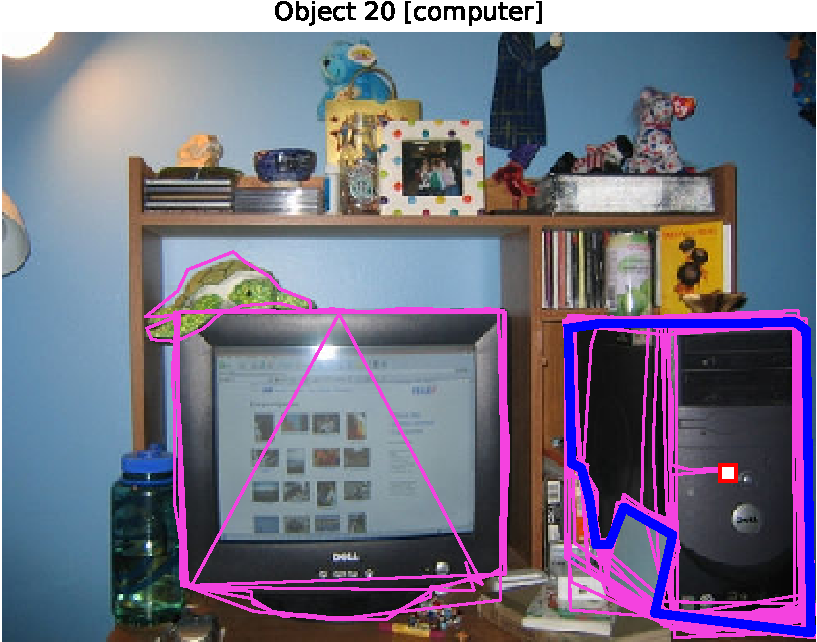
\includegraphics[width=.31\textwidth]{plots/bb_object_20.pdf}
% 	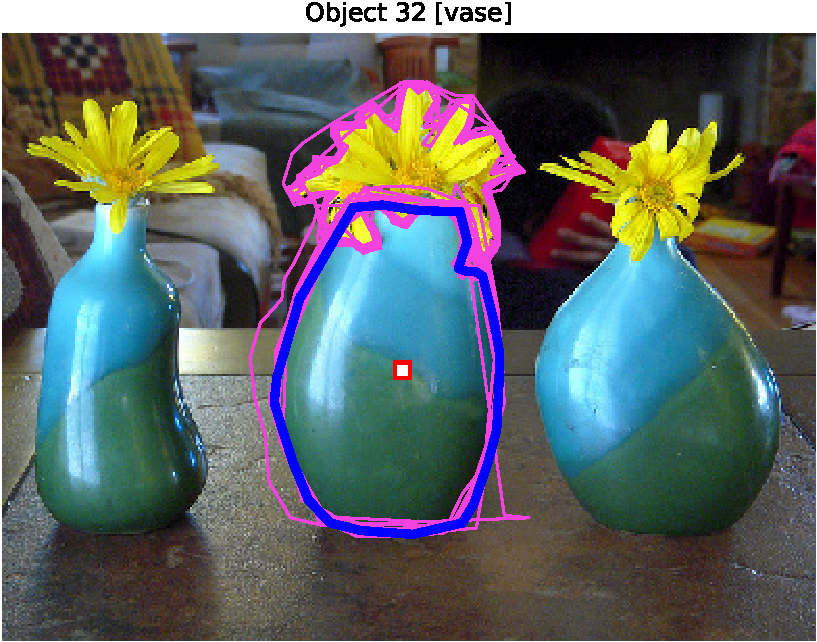
\includegraphics[width=.31\textwidth]{plots/bb_object_32.pdf}
% 	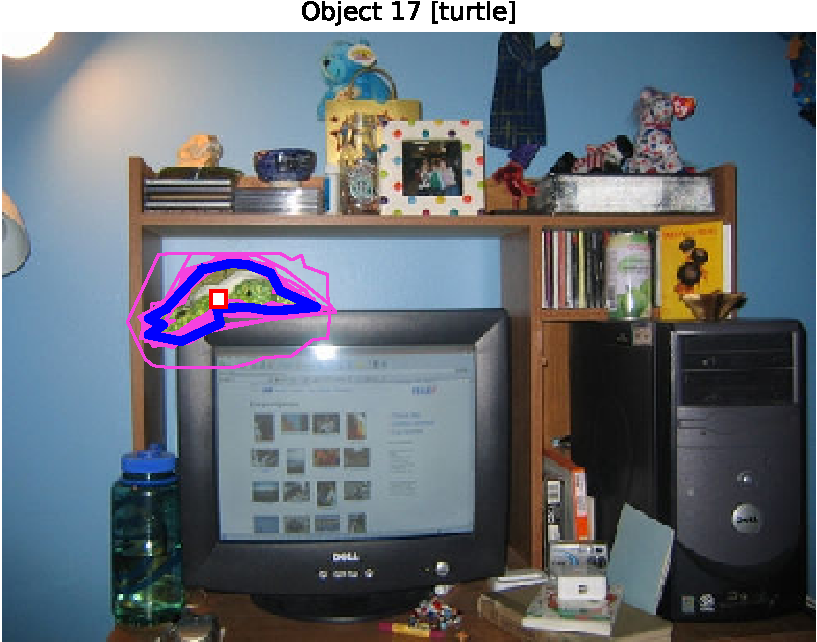
\includegraphics[width=.31\textwidth]{plots/bb_object_17.pdf}
% 	\caption{Pink is the segmentation from individual workers. Blue solid line delineates the ground truth. The red boxed pointer indicates the task of interest shown to users. Examples demonstrating common error patterns among crowdsourced image segmentation, including 1) annotations on the wrong semantic object, 2) ambiguity in regional inclusion and exclusion, and 3) imprecision at the object boundary.}
% 	\label{error_examples}
% \end{figure}
\par As shown in Figure \ref{error_examples}, workers often (i) make unintentional mistakes while drawing the boundaries, either due to low precision of the image, small area of the object, or lack of drawing skills, (ii) have differing opinions about what constitutes the boundary of an object (e.g., is the stalk of a banana part of the fruit?); (iii) or annotate the wrong object entirely (e.g., drawing a bounding box around a dog when the task requests for one around a car). \dor{make the e.g. lines align with what's in the figure.}


Visual examination of worker bounding boxes reveals several common error patterns evident across different objects. As shown in the example in Figure \ref{error_examples}, common worker errors can be classified into three types:
\begin{enumerate}
	\item \textbf{Semantic error:} Workers annotate the wrong semantic object.
	\item \textbf{Regional semantic ambiguity:}Workers annotate the correct semantic object, but included a portion connected to that object that should not have been included as part of the annotation.
	\item \textbf{Boundary imprecision:} Workers annotate the correct semantic object, but segmentation boundaries are imprecise. %(obj 17) \agp{where did obj 7 come from? point to image}
\end{enumerate}
Type 1 and 2 errors have also been observed in prior work~\cite{Sorokin2008,Lin2014,Gurari2018}, which noted that disagreement in worker responses can come from questions that are ambiguous or difficult to answer, such as segmenting a individual person from a crowd. Since there are multiple workers annotating each object, each object can suffer from multiple types of error: we found that out of the 46 objects in our dataset, 9 objects suffer from type one error and 18 objects from type two error. Almost all objects suffer from some form of type three error of varying degree of imprecision around the object boundary. 
\par In the following section, we will first discuss a preprocessing method that we have developed to resolve the multiple worker perspectives found in type one and two errors. Then in the subsequent section, we will described novel aggregation-based algorithms that we have developed and compare them with existing retreival-based methods for addressing type three errors.
As we saw in Section~\ref{sec:errors}, different worker segmentations for the same object can differ from each other due to differences in perspective as well as errors in tracing the outline of the object. Crowdsourcing algorithms need to take these multiple differing worker segmentations as input and output a single, accurate segmentation. 
\subsection{Worker Clustering}
% \subsection{Clustering~\label{sec:clustering}}
Intuitively, workers that have similar perspectives, will have segmentations that are closer to each other, while workers that have different perspectives from each other will have segmentations that differ from each other. We capture the ``similarity'' of a pair of workers by computing the Jaccard coefficient between their segmentations. We perform {\em spectral clustering} to separate workers, using their pairwise similarities, into clusters. We find that the resulting clusters accurately separate and group workers based on their perspectives or the type of semantic errors they make. We also find that the largest cluster is typically free of any semantic errors. Therefore, our preprocessing step consists of clustering workers based on their mutual pairwise Jaccard similarity scores, and filtering away the workers that do not belong to the largest cluster. %\papertext{\todo[inline]{techreport}We omit the details of the clustering algorithm in the interest of space.}\techreport{\todo[inline]{more details}}

Next, we discuss two classes of crowdsourcing algorithms that fundamentally differ in the way they handle multiple worker segmentations to generate a single output segmentation.

